
%(BEGIN_QUESTION)
% Copyright 2010, Tony R. Kuphaldt, released under the Creative Commons Attribution License (v 1.0)
% This means you may do almost anything with this work of mine, so long as you give me proper credit

Determine the ``normal energization'' states (e.g. NE or NDE) of each solenoid valve in this diagram, assuming the process valve needs to be {\it closed} when the process is running as it should:

$$\includegraphics[width=15.5cm]{i04359x01.eps}$$

Also, determine whether one or both solenoids need to ``trip'' in order to make the process valve go to its fail-state.

\vskip 10pt

Suppose the ball valve refused to shut off when it should.  Identify at least two possible faults that could cause this to happen.

\vskip 20pt \vbox{\hrule \hbox{\strut \vrule{} {\bf Suggestions for Socratic discussion} \vrule} \hrule}

\begin{itemize}
\item{} Suppose the probability of each solenoid valve ``sticking'' in its regular operating position instead of tripping when commanded is 6.2 $\times 10^{-3}$.  Calculate the probability of the process valve refusing to trip when commanded as a result of this type of failure.
\item{} Suppose the probability of each solenoid valve ``sticking'' in its tripped position instead of going to its regular operating position when commanded is 7.7 $\times 10^{-3}$.  Calculate the probability of the process valve refusing to go to its regular operating position when commanded as a result of this type of failure.
\item{} Suppose the probability of each solenoid valve accidently tripping during regular operation is 8.1 $\times 10^{-4}$.  Calculate the probability of the process valve tripping accidently as a result of this type of failure.
\end{itemize}

\underbar{file i04359}
%(END_QUESTION)





%(BEGIN_ANSWER)

Both solenoid valves must trip to ``fail'' the process valve (i.e. 2oo2 to trip):

%(END_ANSWER)





%(BEGIN_NOTES)

$$\includegraphics[width=15.5cm]{i04359x02.eps}$$

Possible faults:

\begin{itemize}
\item{} Instrument air supply dead
\item{} Break in tubing between upper solenoid valve and ball valve actuator
\item{} Large leak in ball valve actuator
\end{itemize}

\vskip 10pt

Answers to Socratic Question probability calculations:

$$\includegraphics[width=15.5cm]{i04359x03.eps}$$



















\vskip 20pt \vbox{\hrule \hbox{\strut \vrule{} {\bf Virtual Trip-testing} \vrule} \hrule}

This question is a good candidate for a ``Virtual Trip-testing'' exercise.  Presenting the diagram to students, you pose an assignment whereby students must figure out how to test some component of this system to check that it will operate as intended to shut down the system in an abnormal (trip) condition, with some realistic limitation (e.g. power cannot be shut off to the load).  Students then propose various methods for executing the test.  Your job is to determine whether or not their proposed tests will achieve the desired result(s).

During and after the exercise, it is good to ask students follow-up questions such as:

\begin{itemize}
\item{} Where might our planned test strategy go wrong?  In other words, what thing(s) might happen to foil our test, either to invalidate the results or to not honor the stated limitation(s)?
\item{} Suppose the limitation were different.  How would this affect our ability to carry out the test?
\item{} Is the last test strategy best one we could execute?
\end{itemize}


%INDEX% Final Control Elements, valve: fail-safe solenoids

%(END_NOTES)


